\documentclass{article}

\usepackage{graphicx}
\usepackage{indentfirst}
\usepackage{float}
\usepackage{amsmath,amsfonts,amssymb}
\usepackage[a4paper, total={6in, 8in}]{geometry}
\usepackage{hyperref}
\usepackage{fancyhdr}
\usepackage{xepersian}
\settextfont{B Nazanin}
\setlatintextfont{Times New Roman}


\begin{document}


%title page%
\begin{titlepage}
	\begin{center}
		\textbf{ \Huge{به نام خدا}}	
		\vspace{0.2cm}
		
		
\includegraphics[width=0.4\textwidth]{sharif.png}\\
		\vspace{0.2cm}
		\textbf{ \Huge{آزمایش شماره 3}}\\
		\vspace{0.25cm}
		\textbf{ \Large{آز معماری - دکتر سربازی آزاد}}
		\vspace{0.2cm}
		
		
		\large \textbf{دانشکده مهندسی کامپیوتر}\\\vspace{0.1cm}
		\large   دانشگاه صنعتی شریف\\\vspace{0.2cm}
		\large   ﻧﯿﻢ‌سال اول ۰۰-۰۱ \\\vspace{0.10cm}
		\large{گروه:}\\
		\large{\href{mailto:a.h.hadian@gmail.com}{امیرحسین هادیان - ۹۷۱۰۲۶۰۹}}\\
		\large{\href{mailto:mofayezi.m@gmail.com}{محمدرضا مفیضی - ۹۸۱۰۶۰۵۹}}\\
		\large{\href{mailto:a.hatam008@gmail.com}{علی حاتمی تاجیک - ۹۸۱۰۱۳۸۵}}\\
	\end{center}
\end{titlepage}
%title page%

\newpage

%pages header
\pagestyle{fancy}
\fancyhf{}
\fancyfoot{}
\setlength{\headheight}{59pt}
\cfoot{\thepage}
\lhead{آزمایش شماره 3}
\rhead{
\includegraphics[width=0.1\textwidth]{sharif.png}\\
		دانشکده مهندسی کامپیوتر
}
\chead{آز معماری}
%pages header

\section{هدف}
در این آزمایش قصد طراحی و پیاده سازی یک جمع-تفریق کننده ممیز شناور ۱۲ بیتی داریم. اعداد ورودی نرمالیزه هستند و خروجی نرمالیزه شده خواهد بود. اگر در این فرآیند سرریز رخ بدهد یک خروجی این واقعه را نشان خواهد داد. پس از پایان عملیات نیز سیگنال پایان روشن خواهد شد.
\section{طراحی}
\subsection{\lr{ASM Chart}}
\label{ss:ASMCHART}
طراحی به این صورت است که مدار دارای چهار استیت اصلی است:
\begin{enumerate}
\item ابتدایی:
در این استیت منتظر سیگنال استارت می‌مانیم و زمانی که سیگنال استارت رسید ورودی‌ها را در رجیسترهایی نگه‌داری می‌کنیم تا بتوانیم از آنها در آینده استفاده کنیم تا اگر در ورودی تغییری کردند اشکالی در محاسبات پیش نیاید. 

\item همگام سازی دو عدد:
برای اینکه بتوانیم دو عدد ممیز شناور را با یکدیگر جمع کنیم و یا از هم کم کنیم باید توان برابر داشته باشند. برای همین عددی که توان کمتر دارد را آنقدری شیفت می‌دهیم و به توان آن میافزاییم تا توانها یکسان شوند (عددی که توان بیشتر دارد باارزش تر است).

\item انجام محاسبات:
زمانی که توان‌ها برابر شدند با توجه به اینکه چه عملیاتی باید انجام شود (با توجه به اندازه عدد‌ها و علامت‌ آنها و علملیات درخواست شده) عملیات را روی مانتیس ها انجام می‌دهیم و توان برابر شده در مرحله قبل خواهد بود.

\item نرمال‌سازی:
ممکن است که جواب تولید شده نرمال نباشد که باید نرمال شود. این کار به کمک روشی که در کلاس معماری کامپیوتر معرفی شده است انجام  می‌شود.
\end{enumerate}

چارت نهایی در شکل \ref{asm} آمده است.

\begin{figure}
	\centering
	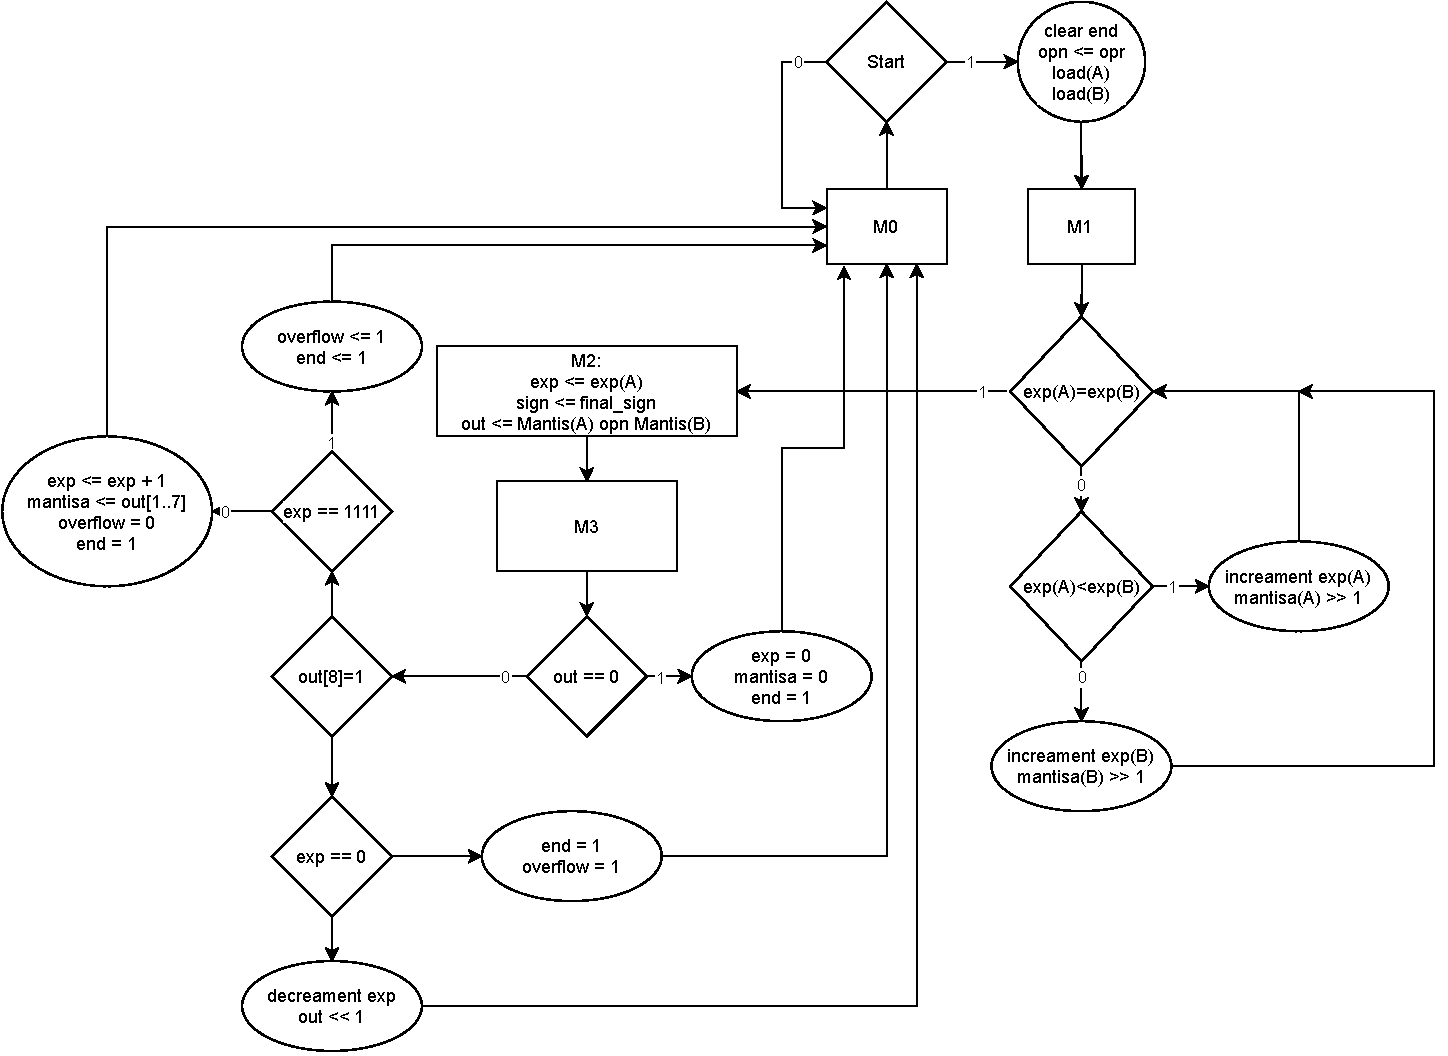
\includegraphics[scale=0.5]{./graphics/asm}
	\caption{چارت}
	\label{asm}
\end{figure}

\subsection{مدار اصلی}
در شکل \ref{base} شمای کلی پیاده‌سازی آمده است. شکل \ref{main} نیز مدار اصلی را نمایش می‌دهد. در ادامه هر بخش آن به صورت مجزا بررسی خواهد شد.

\begin{figure}
	\centering
	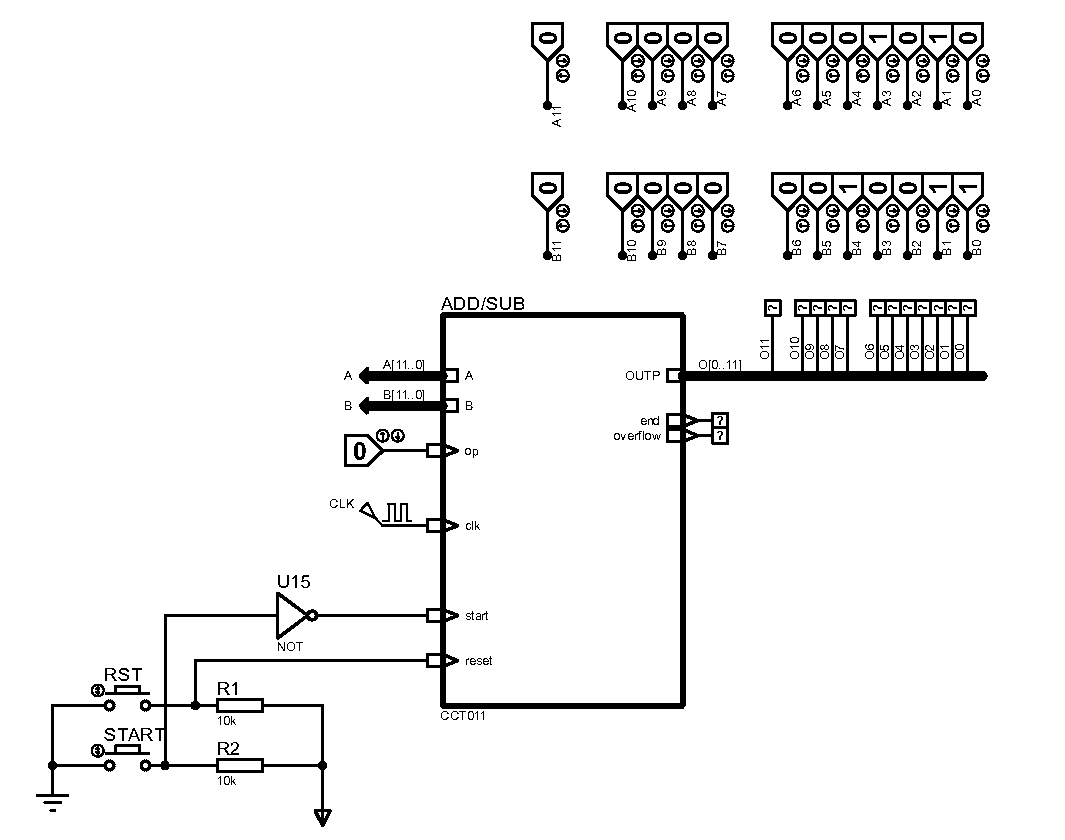
\includegraphics[scale=0.5, page=1]{./graphics/graphics}
	\caption{شمای کلی پیاده‌سازی}
	\label{base}
\end{figure}

\begin{figure}
	\centering
	\includegraphics[scale=0.5, page=2]{./graphics/graphics}
	\caption{مدار اصلی}
	\label{main}
\end{figure}

\subsection{مقایسه کننده}
این بخش یک مدار ترکیبی است که با استفاده از سه مقایسه کننده چهاربیتی ساخته شده است. خروجی این بخش نتیجه مقایسه مانتیس‌ها و توان‌ها را به صورت جداگانه نمایش خواهد داد. به خاطر بداهت طراحی این بخش از توضیحات غیرضروری اجتناب شده است. شماتیک این بخش در شکل \ref{comparator} آمده است. 

\begin{figure}
	\centering
	\includegraphics[scale=0.7, page=6]{./graphics/graphics}
	\caption{واحد مقایسه کننده}
	\label{comparator}
\end{figure}

\subsection{واحد کنترل}
از این بخش می‌توان به عنوان مهم‌ترین بخش مدار یاد کرد. این بخش جابجایی بین استیت‌های مختلف را کنترل می‌کند. ورودی‌های آن شامل سیگنال شروع، سیگنال ریست، نتیجه مقایسه توان‌ها و سیگنال اتمام نرمال‌سازی است. مدار ما شامل چهار استیت است (رجوع شود به \ref{ss:ASMCHART}) که این استیت‌ها به صورت وان‌هات در رجیستر ذخیره می‌شود و خروجی رجیستر نیز به خروجی این ماژول می‌رود. این ماژول سه خروجی دیگر نیز دارد که برای شیفت‌دادن و لود کردن رجیسترهایی که اعداد را نگه‌میدارد استفاده می‌شود. 
با توجه به چارت موجود در بخش \ref{ss:ASMCHART} برای عملیات‌های تغییر استیت خواهیم داشت:

\begin{latin}
\noindent
$M_0^+ = \overline{(M_0+M_1+M_2+M_3)} + \overline{Start}M_0 + Normalize~Fin$\\
$M_1^+ = M_0 Start + \overline{(equal~exp)} M_1$\\
$M_2^+ = M_1(equal~exp)$\\
$M_3^+ = M_2 + M_3\overline{Normalize~Fin}$
\end{latin}

و برای سیگنال‌های کنترل نیز خواهیم داشت (توضیحات کارایی آن در بخش رجیسترها و تعیین علامت آمده است):
\begin{latin}
\noindent
$s_1 = M_0 Satrt$\\
$s_{21} = exp~bigger M_1$\\
$s_{22} = exp~smaller M_1$
\end{latin}

شماتیک واحد کنترل در شکل  \ref{control} آمده است.

\begin{figure}
	\centering
	\includegraphics[scale=0.5, page=4]{./graphics/graphics}
	\caption{بخش رجیستر‌ها}
	\label{control}
\end{figure}

\subsection{رجیستر‌ها}
از بخش \lr{Registers} برای نگه‌داری از ورودی‌ها زمانی که سیگنال استارت می‌خورد استفاده می‌کنیم. این بخش شامل دو تراشه شیفت رجیستر است که مسئولیت نگه‌داری و شیفت دادن احتمالی مانتیس‌‌ها را دارد. همینطور از دو رجیستر با قابلیت انکریمنت نیز برای توان‌ها استفاده می‌کنیم. این بخش علاوه بر سیگنال کلاک و اعداد ورودیمان سه سیگنال کنترلی نیز دریافت می‌کند که عملیات لود و شیفت را کنترل کند. سیگنال $s_1$ در آن برای لود استفاده می‌شود و زمانی که این سیگنال یک باشد لود داده‌ها از ورودی اتفاق می‌افتد. دو سیگنال دیگر هر‌کدام برای کنترل شیفت‌دادن در هر کدام از اعداد هستند. خروجی این بخش دو عدد $A$ و $B$ خواهد بود (اینها با ورودیمان تفاوت دارند و مقادیر داخل رجیسترهایمان هستند). شماتیک این بخش در شکل \ref{registers} آمده است.

\begin{figure}
	\centering
	\includegraphics[scale=0.7, page=5]{./graphics/graphics}
	\caption{بخش رجیستر‌ها}
	\label{registers}
\end{figure}

\subsection{واحد تعیین علامت}
این واحد زمانی که کلید استارت می‌خورد شروع به کار می‌کند. کار آن این است که سه چیز اصلی را مشخص کند: اینکه چه عملیاتی باید بین مانتیس‌ها انجام بگیرد، علامت نهایی چه خواهد بود و اینکه آیا عدد دوم باید عکس شود یا نه (بین مانتیس‌ها فقط جمع انجام می‌گیرد و از این تکنیک برای جمع و تفریق دو مانتیس استفاده می‌کنیم). شماتیک این قسمت از مدار در شکل \ref{operator-sign} آمده است.

\begin{figure}
	\centering
	\includegraphics[scale=0.5, page=7]{./graphics/graphics}
	\caption{تعیین علامت}
	\label{operator-sign}
\end{figure}

\subsection{واحد محاسبات مانتیس}
این واحد با توجه به چیزی که واحد تعیین علامت مشخص کرده است یا مانتیس ها را با یکدیگر جمع میزند و یا اینکه آنها را از هم کم می‌کند. شکل این واحد در شکل \ref{mantis-op} آمده است.
این واحد همچنین دارای دو سیگنال کنترلی است که با توجه به استیتی که در آن هستیم عملیات لود مانتیس را انجام دهد. همینطور زمانی که در نرمال سازی نیاز به شیفت به چپ داریم در این واحد و با سیگنال کنترل شیفت انجام می‌شود. این سیگنال از خروجی‌های واحد محاسبات توان است. 
\begin{figure}
	\centering
	\includegraphics[scale=0.4, page=8]{./graphics/graphics}
	\caption{تعیین علامت}
	\label{mantis-op}
\end{figure}


\subsection{محاسبات توان}
این واحد در دو بخش از محاسبات استفاده می‌شود.
یکی زمانی که در استیت دوم هستیم و باید توان \lr{A }به عنوان توان خروجی ریخته شود و دوم زمانی که در استیت نهایی و مشغول نرمال‌سازی هستیم.
در استیت نهایی هر کجا لازم باشد از توان یکی کم می‌کنیم که معادل با جمع کردن آن با مقدار \lr{1111} است که در واقع همان منفی یک است، و هر کجا لازم باشد آن را شیفت می‌دهیم که با توجه به بیت شماره هشت خروجی و اینکه خروجی صفر نباشد و همچنین استیت تعیین می‌شود.
شکل این واحد در شکل \ref{power} آمده است.
\begin{figure}
	\centering
	\includegraphics[scale=0.6, page=9]{./graphics/graphics}
	\caption{محاسبات توان}
	\label{power}
\end{figure}

\subsection{محاسبه خروجی}
این واحد خروجی نهایی توان و مانتیس و علامت را خروجی می‌دهد تا قابل نمایش باشد.
در صورتی که خروجی صفر باشد، طبق قرار داد تمامی بیت‌های خروجی صفر خواهد شد و در غیر این صورت، تمام ورودی‌ها به خروجی متصل خواهند شد و تنها توان یکی زیاد می‌شود. شکل این واحد در شکل \ref{output} آمده است.

\begin{figure}
	\centering
	\includegraphics[scale=0.5, page=3]{./graphics/graphics}
	\caption{خروجی}
	\label{output}
\end{figure}

\subsection{محاسبات سیگنال‌های خروجی}
در این واحد برخی از سیگنال‌های خروجی لازم برای دیگر واحد‌ها تولید می‌شود.
خروجی \lr{man not zero} زمانی فعال می‌شود که حاصل مانتیس خروجی صفر نباشد و حداقل یک بیت یک در آن وجود داشته باشد.
خروجی \lr{zero} زمانی فعال می‌شود که حاصل مانتیس صفر شده باشد و در استیت نهایی باشیم.
خروجی \lr{normalize fin} زمانی فعال می‌شود که عملیات نرمال کردن تمام شده باشد یا به عبارتی، در استیت نهایی باشیم و بیت نهم یا همان بیت شماره هشت یک شده باشد یا کلا حاصل مانتیس خروجی صفر باشد  یا \lr{underflow} رخ داده باشد.
خروجی \lr{normal} نیز زمانی فعال می‌شود که در استیت نهایی باشیم و بیت شماره هشت خروجی فعال شده باشد و تمامی مقادیر \lr{out} یک نباشد. شکل این واحد در شکل \ref{output-signals} آمده است.

\begin{figure}
	\centering
	\includegraphics[scale=0.6, page=10]{./graphics/graphics}
	\caption{سیگنال‌های خروجی}
	\label{output-signals}
\end{figure}

\subsection{واحد نتیجه}
در این واحد، خروجی‌های \lr{end} و \lr{overflow} محاسبه می‌شوند.
خروجی \lr{end} زمانی فعال می‌شود که که نرمال سازی به اتمام رسیده باشد و مدار در استیت اولیه نباشد.
خروجی \lr{overflow} نیز زمانی فعال می‌شود که بیت پرارزش مانتیس یک شده باشد و مقدار توان نیز حداکثر مقدار خود باشد و دیگر امکان شیفت دادن وجود نداشته باشد.
خروجی \lr{underflow} نیز طبق محاسبات انجام شده است اما چون خواسته‌ی مدار موردنظر در صورت آزمایش نبوده‌است، نشان داده نشده است. شماتیک مدار در شکل \ref{result} آمده است.

\begin{figure}
	\centering
	\includegraphics[scale=0.6, page=11]{./graphics/graphics}
	\caption{واحد نتیجه}
	\label{result}
\end{figure}

\section{تست}
\subsection{جمع دو عدد مثبت}
\begin{figure}[H]
	\centering
	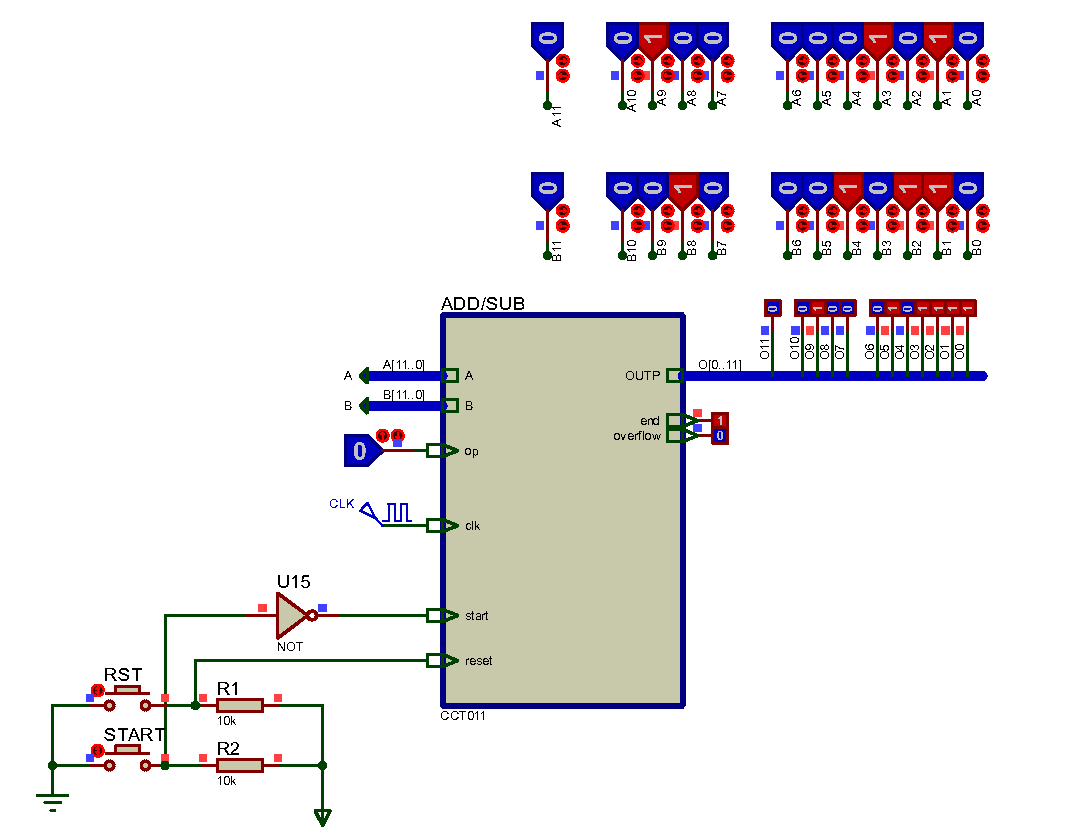
\includegraphics[scale=0.5]{./graphics/tests/PosPlusPos}
\end{figure}

\subsection{تفریق دو عدد مثبت}
\begin{figure}[H]
	\centering
	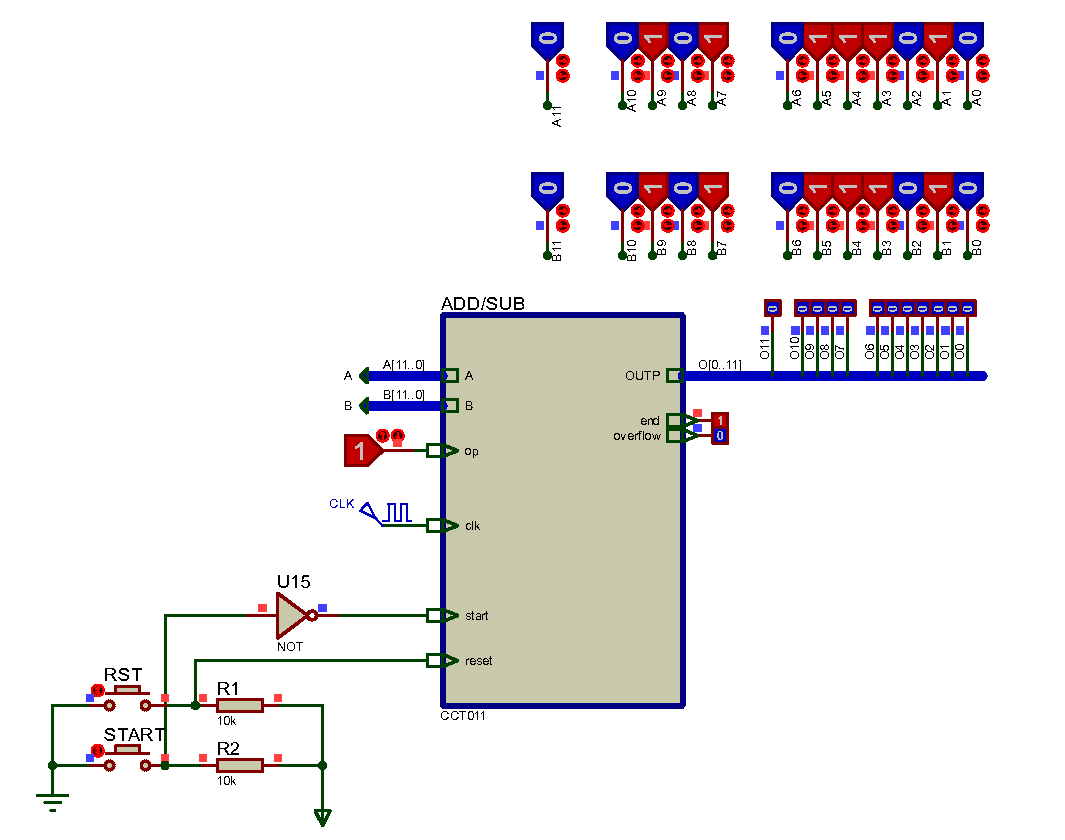
\includegraphics[scale=0.5]{./graphics/tests/PosMinusPosEqual}
\end{figure}


\subsection{جمع دو عدد مختلف‌العلامت}
\begin{figure}[H]
	\centering
	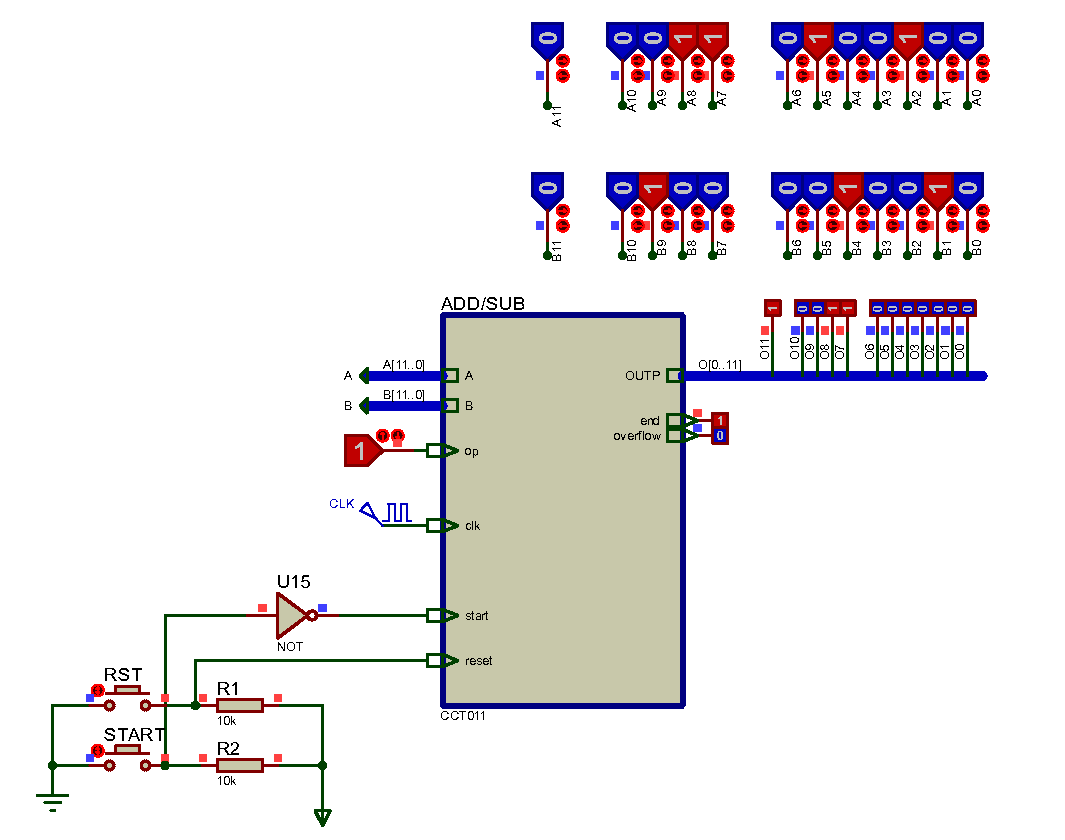
\includegraphics[scale=0.5]{./graphics/tests/PosMinusPosNotEqual}
\end{figure}


\subsection{تفریق دو عدد مختلف‌العلامت}
\begin{figure}[H]
	\centering
	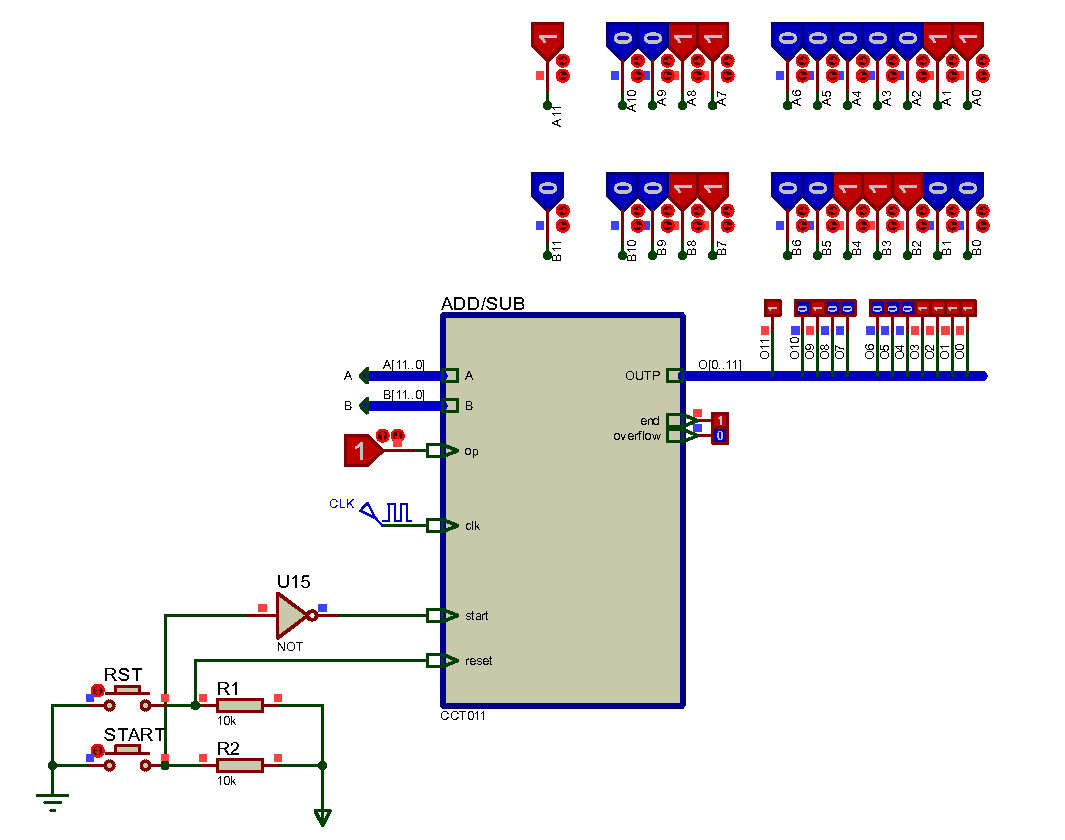
\includegraphics[scale=0.5]{./graphics/tests/subtraction_two_dirrefent_sign_numbers}
\end{figure}


\subsection{تفریق منجر به اورفلو}
\begin{figure}[H]
	\centering
	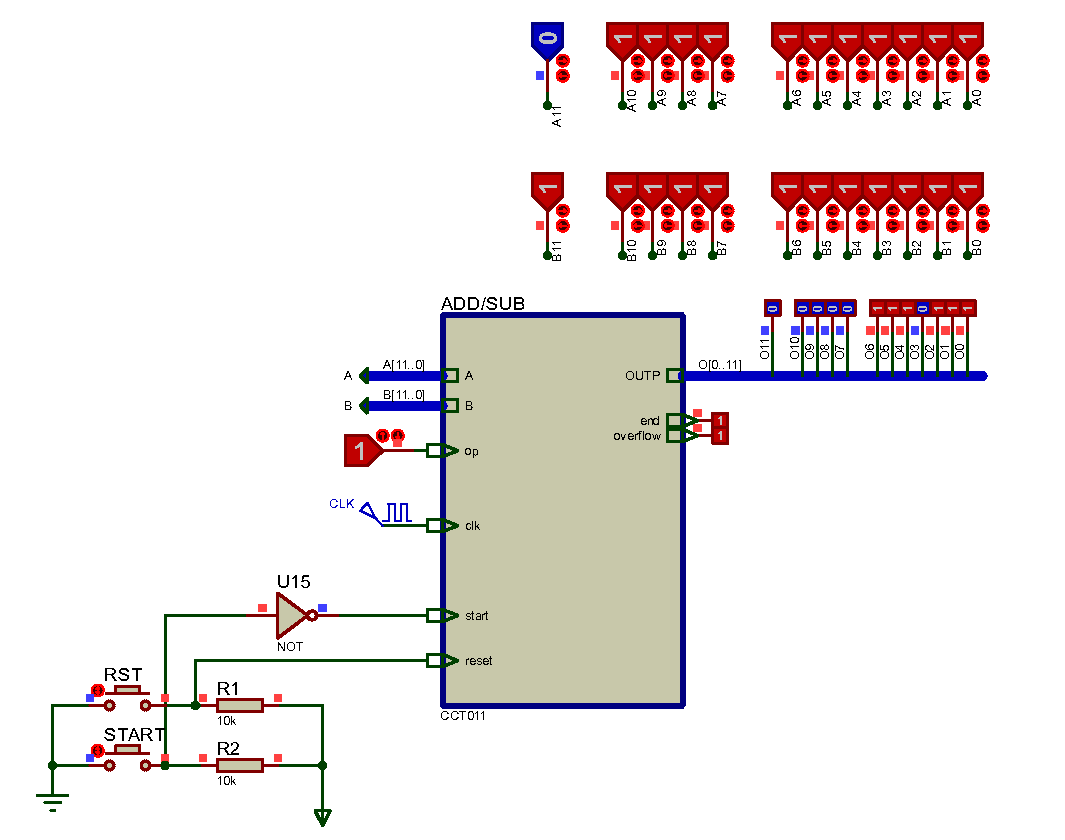
\includegraphics[scale=0.5]{./graphics/tests/subtraction_causing_overflow}
\end{figure}


\subsection{جمع منجر به اورفلو}
\begin{figure}[H]
	\centering
	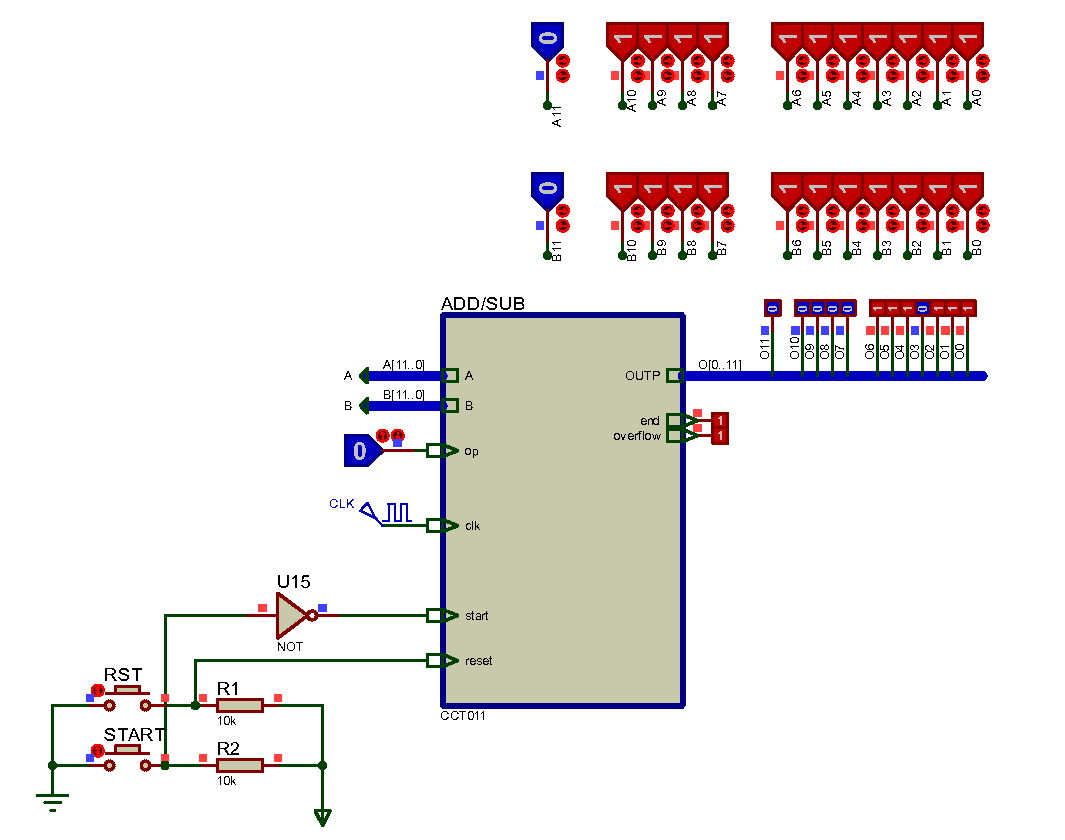
\includegraphics[scale=0.5]{./graphics/tests/addition_causing_overflow}
\end{figure}


\end{document}
